% Main document for Overleaf. Compile with pdfLaTeX and BibTeX.
% The 2017 SIAM class replaces the kernel's label and refstepcounter macros.
% Current hyperref/cleveref need the kernel versions to construct references.
% Restore them before hyperref loads, matching the approach in SIAM's 2025
% class, without changing the requested 2017 class file or its page layout.
\let\siamKernelLabel\label
\let\siamKernelRefstepcounter\refstepcounter
\AddToHook{package/hyperref/before}{%
  \let\label\siamKernelLabel
  \let\refstepcounter\siamKernelRefstepcounter
}

\documentclass[review,onefignum,onetabnum]{siamart171218}
% Title and author information, following the neighboring SIAM Overleaf project.
\usepackage{amsfonts}
\usepackage{amssymb}
\usepackage{amsopn}
\usepackage{booktabs}
\usepackage{graphicx}
\usepackage{tabularx}
\newsiamremark{remark}{Remark}
\headers{QUBO Network Interdiction and Parameter Transfer}{A. Ramesh and D. E. Bernal Neira}
\title{QUBO Network Interdiction with Exact Contraction and QAOA Parameter Transfer}
\author{Anurag Ramesh\thanks{Davidson School of Chemical Engineering,
Purdue University, West Lafayette, IN 47907, USA
(\email{ramesh19@purdue.edu}, \email{dbernaln@purdue.edu}).}
\and David E. Bernal Neira\footnotemark[1]}
\DeclareMathOperator*{\argmin}{arg\,min}
\DeclareMathOperator{\MF}{MF}
\newcommand{\E}{\mathbb{E}}
\newcommand{\bits}{\{0,1\}}
\newcommand{\ket}[1]{\lvert #1\rangle}
\newcommand{\code}[1]{\texttt{\detokenize{#1}}}

\bibliographystyle{siamplain}
\raggedbottom
\emergencystretch=2em
\renewcommand{\footercopyright}{\textcolor{black!50}{Working draft --- 14 October 2026}}
\ifpdf
\hypersetup{pdftitle={QUBO Network Interdiction with Exact Contraction and QAOA Parameter Transfer},
pdfauthor={Anurag Ramesh and David E. Bernal Neira}}
\fi
\begin{document}
\maketitle

\begin{abstract}
Maximum-flow network interdiction selects arcs for removal to reduce the flow between a source and a sink.
We study a quadratic unconstrained binary optimization (QUBO) formulation and a decomposition method for this problem.
The QUBO uses a linear budget term and a quadratic penalty for the cut constraints.
We derive an exact interval for the budget multiplier and a sufficient condition for the cut penalty.
The interval can be empty, so a large multiplier does not always recover the required budget.
We then reduce each piece by an exact contraction of its fixed surroundings.
Budget allocation and repeated piece solves provide a heuristic for the full network.
For the quantum approximate optimization algorithm (QAOA), we compare fixed parameters, two parameter-transfer rules, target-specific training, and a regularized warm start.
A completed statevector experiment uses 12 training graphs and six separate test graphs, with up to 21 qubits.
At depth two, the regularized warm start closes 0.861 of the uniform-to-ground energy gap on average.
The fixed-parameter baseline closes 0.653.
However, energy and optimal-interdiction probability give different rankings, and greedy search solves every test graph exactly.
These results support a reproducible study of formulation and transfer behavior.
They do not establish an advantage on hard interdiction problems.
\end{abstract}

\begin{keywords}
network interdiction, quadratic unconstrained binary optimization, graph contraction,
quantum approximate optimization, parameter transfer, graph attention networks
\end{keywords}
\begin{AMS}
90C27, 90C35, 81P68, 05C21
\end{AMS}

\section{Introduction}\label{sec:introduction}
Network interdiction models the loss of network capacity after an attacker removes selected components.
In maximum-flow interdiction, the attacker has a limited budget and seeks the smallest surviving source-to-sink flow.
The defender then routes as much flow as possible through the remaining network.
The standard formulation uses max-flow/min-cut duality to combine these two decisions into one discrete optimization problem~\cite{wood1993}.

Quantum optimization methods require a further choice of representation.
A QUBO assigns an energy to every binary string, including strings that violate the original constraints.
Its ground states must therefore encode valid interdictions before an energy-based method can solve the intended problem.
Even a correct ground state gives no guarantee that a shallow circuit assigns useful probability to it.
Both formulation correctness and sample quality require separate checks.

This work studies three connected questions.
First, when does the implemented QUBO recover the prescribed interdiction budget?
Second, which parts of a flow network can be removed from a piece subproblem without changing its answer?
Third, can parameters trained on small networks reduce target-specific QAOA training while retaining useful output distributions?
These questions guide the proofs, implementation, and experiments below.

We use established methods as building blocks.
The cut formulation follows classical network interdiction~\cite{wood1993}.
The contraction follows the terminal-cut principle of mimicking networks~\cite{hagerup1998}.
QAOA supplies the parameterized circuit~\cite{farhi2014}.
Graph attention and warm-start methods supply the transfer and initialization tools~\cite{brody2022,egger2021,he2026}.
Our contribution is their explicit specialization to this interdiction QUBO, with exact penalty conditions and a consistent evaluation protocol.
We do not claim that these underlying methods are new.

The current experiments serve different purposes.
Small statevector tests measure parameter transfer on separate weighted graphs.
Larger matrix product state (MPS) simulations test the circuit and sampling pipeline.
The large-network decomposition benchmark remains in progress at this draft's data cutoff.
We report completed data only and keep the limits of each experiment explicit.

\section{Problem and QUBO formulation}\label{sec:formulation}
Let $G=(V,A)$ be a directed graph with distinct source $s$ and sink $t$.
Each arc $a$ has capacity $u_a\geq 0$ and unit interdiction cost.
Let $D\subseteq A$ contain the arcs that can be removed.
The full problem uses $D=A$; a piece subproblem usually uses a strict subset.
An interdiction set $X\subseteq D$ leaves maximum flow $F(X)=\MF(G\setminus X)$.
For an integer budget $0\leq B\leq |D|$, the problem is
\begin{equation}\label{eq:nip}
 f(B)=\min_{X\subseteq D,\ |X|\leq B} F(X).
\end{equation}
Removing an additional arc cannot increase $F$.
Thus an optimal set with exactly $B$ arcs exists whenever $B\leq |D|$.
We also use $f(k)$ for the optimum at each budget $k$.

Let $\pi_i=1$ place vertex $i$ on the source side of a cut.
Fix $\pi_s=1$ and $\pi_t=0$.
For an allowed arc $a=(i,j)\in D$, let $x_a=1$ remove that arc.
The binary variable $\gamma_a$ satisfies
\begin{equation}\label{eq:cut-link}
 \pi_i-\pi_j-\gamma_a\leq 0.
\end{equation}
The cut cost is
\begin{equation}\label{eq:cut-cost}
 C(x,\gamma,\pi)=
 \sum_{a\in D}u_a(1-x_a)\gamma_a
 +\sum_{a=(i,j)\in A\setminus D}u_a\pi_i(1-\pi_j).
\end{equation}
For each fixed $x$, its minimum under \cref{eq:cut-link} equals $F(X)$.
Fixed arcs use the cut expression directly and need no $x$, $\gamma$, or auxiliary variable.

\subsection{Quadratic cut penalty}
The cut constraint fails only at $(\pi_i,\pi_j,\gamma_a)=(1,0,0)$.
Introduce one binary auxiliary variable $w_a$ and define
\begin{equation}\label{eq:penalty}
 P_a=\pi_j\gamma_a-\pi_j-\gamma_a
       +w_a(\pi_i+\pi_j+\gamma_a-1).
\end{equation}
For a budget multiplier $\lambda\geq 0$ and cut penalty $\eta>0$, the QUBO is
\begin{equation}\label{eq:qubo}
 Q=C(x,\gamma,\pi)+\lambda\left(\sum_{a\in D}x_a-B\right)
           +\eta\sum_{a\in D}P_a.
\end{equation}
It uses $|V|-2+3|D|$ logical binary variables before any additional simplification.
For the full graph, this count is $|V|-2+3|A|$.
The budget term is linear and can be negative below budget.
It is a Lagrangian term, not a squared constraint penalty.

\begin{lemma}\label[lemma]{lem:quadratization}
For each fixed $(\pi_i,\pi_j,\gamma_a)\in\bits^3$,
\[
 \min_{w_a\in\bits}P_a=\pi_i(1-\pi_j)(1-\gamma_a)-1.
\]
\end{lemma}
\begin{proof}
If $\pi_j=\gamma_a=0$, the minimum is $\min\{0,\pi_i-1\}$.
It equals $0$ when $\pi_i=1$ and $-1$ when $\pi_i=0$.
Otherwise, the first three terms in \cref{eq:penalty} equal $-1$.
The coefficient of $w_a$ is then nonnegative, so $w_a=0$ attains the minimum.
These cases give the stated identity.
\end{proof}

\begin{proposition}\label[proposition]{prop:dual-penalty}
If $\eta>\lambda\geq0$, every ground state of \cref{eq:qubo} satisfies all cut constraints.
After joint minimization, the ground energy is
\begin{equation}\label{eq:ground-general}
 E_* = \min_{0\leq k\leq |D|}\{f(k)+\lambda(k-B)\}-\eta|D|.
\end{equation}
\end{proposition}
\begin{proof}
Each auxiliary variable can first minimize its own penalty without changing any other term.
Suppose arc $a$ violates \cref{eq:cut-link}.
Set $x_a=\gamma_a=1$ and minimize $w_a$ again.
The cut cost on $a$ is zero before and after this change.
The budget term increases by at most $\lambda$, and the cut penalty decreases by $\eta$.
All other arc constraints stay unchanged.
The total energy strictly decreases, so a ground state cannot contain a violation.
The minimum feasible cut cost at cardinality $k$ is $f(k)$.
Every satisfied cut constraint contributes $-\eta$ after auxiliary minimization, which gives \cref{eq:ground-general}.
\end{proof}

The implementation sets $\eta=\lambda+1$ in the numerical capacity units of each instance.
The proof applies to the joint minimum over interdictions and cuts.
It does not assert that every infeasible string has greater energy than every feasible string.
It also does not justify $\eta>\lambda$ as a sufficient condition when an arbitrary $x$ is held fixed.
For that stronger fixed-$x$ statement, $\eta>\max_{a\in D}u_a$ is sufficient.

\subsection{Exact interval for the budget multiplier}
For an interior budget $0<B<|D|$, define
\begin{equation}\label{eq:window}
 L_B=\max_{k>B}\frac{f(B)-f(k)}{k-B},
 \qquad
 U_B=\min_{k<B}\frac{f(k)-f(B)}{B-k}.
\end{equation}

\begin{theorem}\label{thm:window}
Assume $\eta>\lambda\geq0$.
Every ground state of \cref{eq:qubo} uses exactly $B$ arcs and attains $f(B)$ if and only if
\begin{equation}\label{eq:strict-window}
 L_B<\lambda<U_B.
\end{equation}
In this case, $E_*=f(B)-\eta|D|$.
Replacing the strict inequalities by non-strict inequalities permits ties with other budgets.
\end{theorem}
\begin{proof}
By \cref{prop:dual-penalty}, ground-state cardinalities minimize $f(k)+\lambda k$.
Exactly $B$ is the unique minimizing cardinality if and only if
\[
 f(B)+\lambda B<f(k)+\lambda k\qquad(k\neq B).
\]
For $k>B$, each inequality is a lower bound on $\lambda$.
For $k<B$, it is an upper bound.
Their intersection is \cref{eq:strict-window}.
\end{proof}

The condition depends on changes in optimal flow, rather than individual arc capacities.
A nonempty interval exposes $(B,f(B))$ as a strict vertex of the lower convex envelope of the cardinality curve.
If the interval is empty, no nonnegative linear multiplier isolates that budget.
An arbitrarily large multiplier instead favors smaller interdiction sets.

Our implementation computes the curve with exact interdiction solves and chooses an interior multiplier when one exists.
It rejects an empty interval.
This procedure gives a reference construction for experiments, but the exact solves can be expensive.
Parameter transfer does not remove that cost.
For example, the small instance \code{tiny_b} has $f(k)=(25,13,5,0)$ until flow vanishes.
At $B=1$, the exact interval is $(8,12)$.
Choosing $\lambda=6$ favors two removed arcs and violates the intended budget.

\section{Decomposition with exact contraction}\label{sec:decomposition}
We partition the vertices into pieces and assign each directed arc to the piece containing its tail.
This ownership rule gives each removable arc exactly one budget allocation.
The implementation recursively applies Kernighan--Lin bisection to the undirected graph and separates disconnected parts~\cite{kernighan1970}.
The partition ignores capacity weights.
It controls the number of local decision variables, but does not guarantee balanced QUBO sizes.

\subsection{Contraction of a fixed region}
Consider one active piece.
Other interdictions are fixed during its solve.
Let $Z$ contain the vertices outside the piece, and let $T$ contain its boundary vertices and any global terminals in $Z$.
The internal arcs of $Z$ cannot change during this solve.
For each allowed assignment $\ell:T\to\bits$, define $g(\ell)$ as the minimum internal cut capacity under those labels.
Labels at $s$ and $t$, when present, remain fixed.

Choose one minimum cut for each assignment $\ell$.
Record the side of every vertex in every chosen cut.
Merge vertices with identical records, sum parallel arc capacities, and discard self-loops.
This construction is a terminal-cut form of a mimicking network~\cite{hagerup1998}.

\begin{proposition}\label[proposition]{prop:contraction}
The contracted region has the same value $g(\ell)$ for every allowed terminal assignment.
It therefore preserves the full network's maximum flow under every interdiction outside the internal arcs of $Z$.
\end{proposition}
\begin{proof}
A cut of the contracted region lifts to a cut of the original region with equal capacity.
Contraction thus cannot decrease the minimum for a fixed assignment.
Conversely, no merged class crosses any recorded minimum cut.
That cut survives contraction and retains value $g(\ell)$.
The two minima are equal.
In the full network, fix the labels at the boundary and minimize the internal and external cut contributions.
The internal contribution is unchanged for each boundary assignment.
Minimizing over those assignments proves the final statement by max-flow/min-cut duality.
\end{proof}

With $r$ free terminal labels, construction requires $2^r$ minimum-cut computations.
The implementation uses $r\leq12$ by default.
Above that limit, it retains the original region and preserves correctness without reducing its size.
It also retains the original identity of every removable arc.
Thus local solutions map back to valid arcs of the full network.

Exactness depends on the internal arcs being fixed.
If the region can use a positive interdiction budget during the same solve, its cut function depends on those decisions.
A contraction computed before those decisions need not preserve the result.
We therefore claim exact reduction only for the fixed surroundings of an active piece.

\subsection{Budget allocation and repeated solves}
Let $b_i$ be the budget of piece $i$, with $\sum_i b_i=B$.
Two initial rules distribute budget in proportion to minimum-cut arc counts or local flow estimates.
Largest-remainder apportionment makes the budgets integral, with caps from the number of owned arcs.
A third rule solves local cardinality curves $f_i(k)$ in the intact network.
It chooses budgets by the dynamic program
\begin{equation}\label{eq:allocation}
 \max_{b_1+\cdots+b_m=B}\sum_{i=1}^m\{f_i(0)-f_i(b_i)\}.
\end{equation}
The objective treats local flow reductions as additive.
Interactions among pieces can break that assumption, so this allocation is a heuristic.

Independent solves choose each piece's cuts in the intact network.
Sequential solves fix earlier choices before solving the next piece.
Repeated sequential passes accept a replacement only when it reduces the full network's surviving flow.
The implementation allows ten such passes by default.
An optional refinement transfers one budget unit between two pieces and keeps an improvement, for at most twenty steps.
These rules preserve feasibility and prevent accepted refinements from worsening flow.
They do not certify the global interdiction optimum.

For each reduced graph, only owned arcs receive interdiction variables.
The remaining arcs contribute their fixed cut cost as in \cref{eq:cut-cost}.
The piece QUBO therefore uses $|V_i'|-2+3|D_i|$ variables.
The partition search checks this actual count against a requested qubit limit.
It records failure when no tested partition fits.
A small piece alone is insufficient if its surroundings have many terminals and remain uncontracted.

\section{QAOA and parameter transfer}\label{sec:qaoa}
Map each QUBO variable $y_j$ to $(1-Z_j)/2$.
The resulting diagonal Hamiltonian is
\begin{equation}\label{eq:ising}
 H=c_0 I+\sum_j h_jZ_j+\sum_{j<k}J_{jk}Z_jZ_k.
\end{equation}
Let $c=\max\{|h_j|,|J_{jk}|\}$ over nonzero coefficients.
We train circuits on $\widetilde H=(H-c_0I)/c$ and retain this convention for every donor and target.
This normalization makes angle transfer well defined across different coefficient scales.
It does not make distinct Hamiltonians equivalent.

Standard QAOA starts from $\ket{+}^{\otimes n}$~\cite{farhi2014}.
At each layer $\ell$, it applies $\exp(-i\gamma_\ell\widetilde H)$, followed by $\exp(-i\beta_\ell\sum_jX_j)$.
The stored parameter vector is $(\beta_1,\ldots,\beta_p,\gamma_1,\ldots,\gamma_p)$.
COBYLA trains this vector from a fixed ramp initialization.
Each donor bank contains one depth and one normalization convention.

\subsection{Flow features and donor selection}
We compute features on the directed flow network.
Node features identify the source and sink and describe incoming and outgoing degree and capacity.
Arc features contain scaled capacity, message direction, and whether the arc can be interdicted.
Graph features include size, relative budget, the multiplier, and capacity statistics.
\Cref{sec:features} specifies them.
The multiplier and capacity scale matter because the cut penalty is $\lambda+1$.

The nearest-donor rule uses the IBM QAOA training pipeline with our feature extractor and matching function~\cite{ibmpipeline}.
It divides each graph feature by its standard deviation in the training set.
It then selects the closest training vector in Euclidean distance and returns that donor's angles.
Constant features use scale one, and donor order breaks ties.
This is a deterministic nearest-neighbor baseline; the IBM interface does not add a second learned model.

The graph attention network (GAT) chooses from representative donor schedules.
Its training procedure adapts the released QAOA transfer implementation for maximum independent set~\cite{gattransfer}.
We replace its problem features with the flow features above and use GATv2 layers~\cite{brody2022}.
Three layers produce 32 features per node.
Mean pooling and the graph features feed a two-layer classifier.

To choose representatives, evaluate every donor schedule on every training graph.
For training target $i$ and donor $j$, record
\begin{equation}\label{eq:profile}
 M_{ij}=\langle\widetilde H_i\rangle_{\theta_j}/n_i.
\end{equation}
Ward clustering groups the donor columns into four clusters.
The medoid of each cluster supplies one representative schedule.
The best representative energy on each training graph supplies its class label.
We fit the classifier with cross-entropy loss and Adam for 200 epochs.
The learning rate is $0.005$ and the dropout probability is $0.2$.
Inference uses no target circuit evaluations or target optimum as a feature.
However, problem construction still uses the exact multiplier procedure from \cref{sec:formulation}.

\subsection{Regularized warm start}
Warm-start QAOA uses a classical solution to define a product state and a matching mixer~\cite{egger2021}.
We adapt the regularized product-state approach of He et al.~\cite{he2026} to the full interdiction Hamiltonian, including its linear terms.
For $z\in[-1,1]^n$, solve
\begin{equation}\label{eq:rws}
 \min_z\left\{
  \frac{\sum_jh_jz_j+\sum_{j<k}J_{jk}z_jz_k}{c}
  +\rho\sum_jz_j^2\right\}.
\end{equation}
Here $\rho=0.6$ is dimensionless and differs from the budget multiplier $\lambda$.
The positive regularizer favors values away from fully polarized endpoints.
We use L-BFGS-B from zero and three seeded random starts, and retain the best converged result.
This local optimization gives no global certificate for \cref{eq:rws}.

Set $\alpha_j=\arccos z_j$ and prepare $\bigotimes_j R_y(\alpha_j)\ket{0}$.
Use the mixer
\begin{equation}\label{eq:warm-mixer}
 H_M=\sum_j\bigl(\sin\alpha_jX_j+\cos\alpha_jZ_j\bigr).
\end{equation}
The implementation applies its one-qubit exponential with the ordered gates
$R_y(-\alpha_j)$, $R_z(2\beta)$, and $R_y(\alpha_j)$.
We train one shared angle schedule by minimizing mean normalized energy per qubit over the training graphs.
Each test graph receives that fixed schedule and its own classical product-state optimization.
Thus this method avoids target quantum-angle training but retains target classical setup work.
Our interdiction experiment is an adaptation, not a replication of the Max-Cut results in~\cite{he2026}.

\subsection{Use within decomposition}
The transfer adapter builds the restricted piece QUBO, selects donor angles, samples the circuit, and repairs the sampled interdictions.
It permits only arcs owned by that piece and maps them back to the full graph.
A zero-budget piece returns no interdictions.
An empty multiplier interval or an exceeded qubit limit produces an explicit failure.
A saved-model integration check solves a contracted piece of \code{tiny_a} and returns flow $5$, the exact optimum.
This check establishes compatibility of the components.
A complete large-network comparison with transferred piece solvers remains future work.

\section{Experimental protocol}\label{sec:protocol}
\subsection{Measures and classical references}
We evaluate every interdiction by maximum flow on the original network.
Exact enumeration supplies small-instance references; larger references use the Gurobi formulation.
Greedy search starts with no cuts and repeatedly removes the arc with the largest immediate flow reduction.
Sample repair adds or restores arcs by their flow effect until the budget is met.
For piece subproblems, both steps respect the allowed arc set.

For a nontrivial instance, define the flow-reduction ratio
\begin{equation}\label{eq:flow-ratio}
 R(X)=\frac{F(\varnothing)-F(X)}{F(\varnothing)-f(B)}.
\end{equation}
A feasible optimum has ratio one.
This ratio measures the original task, while QUBO energy also measures cut and auxiliary-variable consistency.
We report repaired flow separately because repair can supply much of the observed improvement.

The uniform computational-basis distribution has mean energy $E_{\mathrm{unif}}=c_0$.
We measure normalized energy improvement by
\begin{equation}\label{eq:gap}
 G_E=\frac{c_0-\langle H\rangle}{c_0-E_*}.
\end{equation}
It equals zero for the uniform reference and one at the ground energy.
This measure avoids an energy ratio whose additive offset can make uniform output appear strong.
It need not be nonnegative for an arbitrary circuit.

The optimal-interdiction probability $P_{\mathrm{opt}}$ counts exactly-$B$ interdictions with flow $f(B)$, regardless of cut or auxiliary bits.
It differs from full ground-state probability.
The budget-feasible fraction $P_{\mathrm{feas}}$ counts sampled interdictions using at most $B$ arcs.
We decode up to twenty distinct low-energy samples for repair and report the best repaired flow.
All experiments below use 4096 samples per circuit and seed zero.

\subsection{Separate training and test graphs}
The transfer experiment uses twelve four-vertex training graphs and six five-vertex test graphs.
Each graph has two directed source-to-sink routes, with an optional cross arc.
Capacities are independent integer draws from 1 through 20 before rejection.
We reject duplicate weighted graphs and graphs without a strict budget-one multiplier interval.
This conditioning limits the population to which the results apply.
It also makes the exact multiplier information part of the experimental setup.

Training circuits use 14 or 17 qubits.
Test circuits use 18 or 21 qubits.
The largest dense state contains $2^{21}=2{,}097{,}152$ complex amplitudes.
At sixteen bytes per amplitude, the state alone needs 32 MiB; operators, probabilities, and simulator workspaces add memory.
These runs use classical statevector simulation, with no device noise.

At depths $p=1,2$, compare five methods on the same six test graphs.
They are target-specific COBYLA, the first donor's fixed schedule, nearest-donor transfer, GAT transfer, and the regularized warm start.
COBYLA has a limit of 150 objective evaluations per fit.
All donor schedules and fitted model parameters come from training graphs.
Target graph features guide donor selection.
The six test graphs share a structural family with the training set and have one extra vertex.
They test limited size transfer, not transfer across graph families.

Each graph has $B=1$.
Greedy search then enumerates all one-arc removals and is exact by construction.
This experiment can compare quantum distributions and training costs, but cannot demonstrate a better interdiction solution than greedy search.
One graph split and one seed provide descriptive evidence, without a statistical generalization claim.

\subsection{Mid-size MPS cohort}
The second cohort has 23 valid instance-budget pairs from nine planar, Erd\H{o}s--R\'enyi, and nearest-neighbor graphs.
The QUBOs have 39--149 qubits.
We simulate depths one through three with Aer MPS and maximum bond dimension 32.
A fixed schedule from the tiny-instance study is evaluated on all 23 pairs.
Target-specific training is available for ten pairs with at most 81 qubits.
This gives 99 completed rows.

We compare the trained and donor schedules only on their common ten pairs.
An average over all donor rows would compare different problem sizes.
The bond cap makes these MPS calculations approximate.
No bond-dimension convergence study is included, so we do not treat their energies as exact circuit values.
Greedy search reaches the exact interdiction optimum on all 23 pairs.

\section{Completed results}\label{sec:results}
\subsection{Statevector parameter transfer}
\Cref{tab:transfer} reports means over the six test graphs.
At depth one, the regularized warm start closes $0.7967$ of the uniform-to-ground gap.
At depth two, it closes $0.8610$.
The corresponding fixed-donor values are $0.4941$ and $0.6528$.
The warm start also produces much larger budget-feasible fractions in this cohort.

\begin{table}[tb]
\centering
\small
\caption{Statevector comparison. Each row averages the same six held-out graphs. $P_{\mathrm{opt}}$ uses exact state probabilities; $P_{\mathrm{feas}}$ uses 4096 sampled bit strings. Evaluations count target quantum-angle optimizer calls.}
\label{tab:transfer}
\begin{tabular}{llrrrr}
\toprule
$p$ & Method & $G_E$ & $P_{\mathrm{opt}}$ & $P_{\mathrm{feas}}$ & Evaluations \\
\midrule
1 & Fixed donor & 0.4941 & 0.0689 & 0.2013 & 0.0 \\
1 & Nearest donor & 0.4947 & 0.0684 & 0.1978 & 0.0 \\
1 & GAT & 0.4894 & 0.0676 & 0.2092 & 0.0 \\
1 & Target trained & 0.5004 & 0.0677 & 0.2008 & 31.7 \\
1 & Warm start & 0.7967 & 0.1428 & 0.8062 & 0.0 \\
\midrule
2 & Fixed donor & 0.6528 & 0.1322 & 0.4033 & 0.0 \\
2 & Nearest donor & 0.6511 & 0.1342 & 0.4003 & 0.0 \\
2 & GAT & 0.6621 & 0.1283 & 0.4043 & 0.0 \\
2 & Target trained & 0.6695 & 0.1377 & 0.4062 & 100.5 \\
2 & Warm start & 0.8610 & 0.1183 & 0.8693 & 0.0 \\
\bottomrule
\end{tabular}
\end{table}


GAT and nearest-donor transfer remain close to the fixed donor in mean energy.
At depth two, GAT closes $0.6621$ of the gap, compared with $0.6695$ for target-specific COBYLA.
This small difference does not establish equivalence or superiority.
The comparison contains only six graphs and no repeated training splits.
The per-graph values in \cref{fig:transfer} show the variation hidden by the means.

\begin{figure}[tb]
\centering
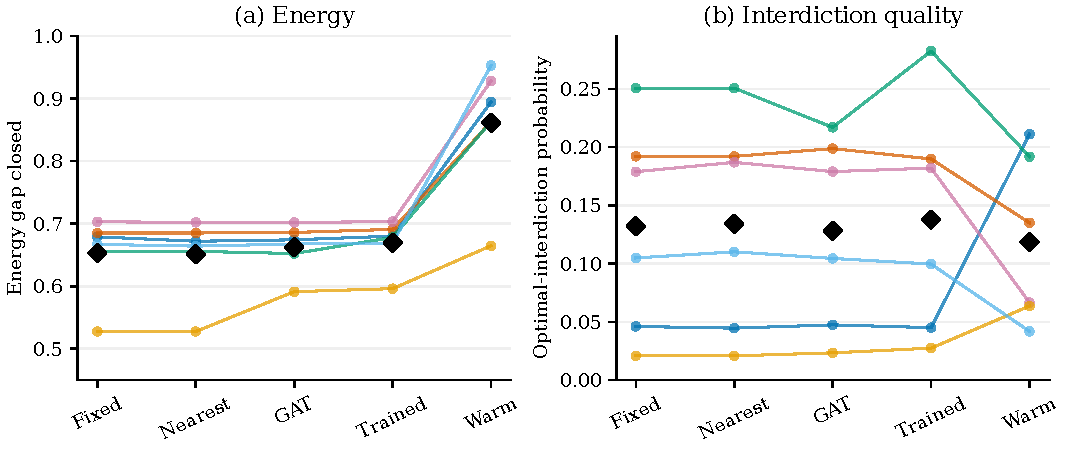
\includegraphics[width=\linewidth]{figures/transfer_depth_two.pdf}
\caption{Depth-two results on all six held-out graphs. Each connected line is one graph; black diamonds show the means.
Energy improvement and optimal-interdiction probability measure different properties of the output distribution.
The graph order and data are identical in both panels.}
\label{fig:transfer}
\end{figure}

Energy improvement does not imply a larger probability of optimal interdiction.
At depth two, the warm start has $P_{\mathrm{opt}}=0.1183$ on average.
The target-trained standard circuit has $P_{\mathrm{opt}}=0.1377$.
The warm-start energy objective rewards all Hamiltonian terms, including cut and auxiliary consistency.
The optimal-interdiction event ignores those auxiliary decisions.
The different rankings are therefore consistent with the definitions.

Every method reaches the exact optimum after repair on all test graphs.
Because greedy search is also exact here, repaired flow does not separate the methods.
An ablation with the initial warm product state alone is still needed to isolate the contribution of its QAOA layers.
This draft therefore attributes the measured scores to the complete warm-start procedure.

Transferred schedules use zero target quantum-angle optimization evaluations.
Target-specific COBYLA averages 31.7 evaluations at depth one and 100.5 at depth two.
The corresponding mean optimizer times are 34.0 and 136.5 seconds in this run.
Donor-bank training costs 19.1 and 77.5 seconds, while GAT construction and fitting cost 8.2 and 9.2 seconds.
The pooled warm-start schedules cost 24.0 and 78.6 seconds to construct and train.
These timings exclude several costs, including initial exact-reference construction, and come from a shared machine.
They measure components of this implementation, not an end-to-end speedup.

\subsection{Paired MPS results}
On the ten common instance-budget pairs, trained schedules improve the mean energy measure at each depth.
\Cref{tab:mid} also shows higher sampled feasibility and optimal-interdiction frequency.
At depth three, training raises mean $G_E$ from $0.6853$ to $0.7589$ and mean $P_{\mathrm{feas}}$ from $0.2061$ to $0.4362$.
These results describe the bond-32 simulation and require a convergence study before stronger circuit-level conclusions.

\begin{table}[tb]
\centering
\small
\caption{Paired MPS comparison on ten instance-budget pairs with at most 81 qubits. The maximum bond dimension is 32. Both probabilities are sampled estimates. The last column counts optimal repaired solutions.}
\label{tab:mid}
\begin{tabular}{llrrrr}
\toprule
$p$ & Schedule & $G_E$ & $P_{\mathrm{opt}}$ & $P_{\mathrm{feas}}$ & Repaired \\
\midrule
1 & Donor & 0.4392 & 0.0007 & 0.0065 & 9/10 \\
1 & Target trained & 0.5260 & 0.0017 & 0.0142 & 10/10 \\
2 & Donor & 0.5879 & 0.0070 & 0.0481 & 10/10 \\
2 & Target trained & 0.6654 & 0.0153 & 0.1403 & 10/10 \\
3 & Donor & 0.6853 & 0.0253 & 0.2061 & 9/10 \\
3 & Target trained & 0.7589 & 0.0379 & 0.4362 & 10/10 \\
\bottomrule
\end{tabular}
\end{table}


Across all 99 rows, 28 rows contain no budget-feasible sample.
Target-trained schedules nevertheless reach the exact optimum after repair on all thirty trained rows.
Greedy search also reaches that optimum on every instance-budget pair.
The distinction between raw sampling and repair is therefore essential for this cohort as well.

\subsection{Decomposition results pending}
The large-network benchmark evaluates 27 instance-budget pairs with two partition settings.
It compares three budget rules and independent, sequential, and repeated solves, with an additional budget-refinement variant.
The piece solver in that benchmark is classical Gurobi.
Each piece solve uses eight Gurobi threads.
Partitioning and contraction use separate serial NetworkX operations.
The benchmark starts from the first case under this fixed thread budget; it does not combine timings from earlier runs.
Its full output is not yet complete at this draft's cutoff of 14 October 2026.
We omit partial performance tables to avoid favoring the graph families that finished first.
The exact contraction result in \cref{prop:contraction} does not depend on completion of this benchmark.

\section{Discussion and remaining experiments}\label{sec:discussion}
The current formulation gives a precise test for whether a linear budget multiplier can work.
The cut penalty has a simple sufficient condition, but the budget multiplier has both a lower and an upper limit.
An empty interval requires a different budget encoding or a method that handles budget feasibility directly.
Finding the interval through exact cardinality solves is useful for verification, but limits the present solver's practical role.

Contraction reduces fixed surroundings without changing local answers.
Its cost depends exponentially on the number of boundary terminals, so separator quality matters.
The outer decomposition still needs evidence on global solution quality and total runtime.
The pending benchmark will supply the first full comparison of its budget and update rules.
A later experiment must assess transferred QAOA piece solvers on the same networks and budgets.

Parameter transfer reduces target quantum-angle training in the completed small experiment.
The learned GAT does not show a consistent advantage over the simpler donor baselines in the reported means.
The warm start changes both the initial state and the mixer, so its improvement cannot be assigned to angle transfer alone.
The next study should add a product-state-only baseline, multiple graph splits, multiple optimizer starts, and matched compute budgets.

Harder interdiction instances are also necessary.
They should include budgets greater than one, interior optimal cuts, and cases where greedy search has a measured optimality gap.
The experiment should report exact-reference cost, contraction cost, model training, inference, circuit sampling, and repair separately.
For MPS, increasing bond dimensions must test convergence.
For hardware, device noise and compilation costs require a separate evaluation.
No hardware performance claim is made from the simulations in this draft.

\section{Conclusion}
We give exact penalty conditions for a network-interdiction QUBO and an exact contraction for fixed regions of a flow network.
These results define which parts of the combined method preserve the original optimization problem.
Budget allocation and QAOA sampling remain heuristic components.
The completed experiments provide reproducible comparisons of parameter transfer, warm starts, and target-specific training.
They also show why energy, feasibility, optimal-interdiction probability, and repaired flow must be reported separately.
Establishing value on hard interdiction problems requires the larger comparisons and ablations described above.

\appendix
\section{Feature definitions}\label{sec:features}
Let $n=|V|$, $m=|A|$, $d=|D|$, and $U=\max\{1,\max_a u_a\}$.
Let $q_i^{\mathrm{in}}$ and $q_i^{\mathrm{out}}$ denote the total incoming and outgoing capacity at vertex $i$.
The six node features are
\[
 \left(\mathbf{1}_{i=s},\mathbf{1}_{i=t},
 \frac{\deg^-(i)}{\max(n-1,1)},\frac{\deg^+(i)}{\max(n-1,1)},
 \frac{q_i^{\mathrm{in}}}{Um},\frac{q_i^{\mathrm{out}}}{Um}\right).
\]
Each original arc sends a forward and a reverse message.
Their features are $(u_a/U,+1,\mathbf{1}_{a\in D})$ and $(u_a/U,-1,\mathbf{1}_{a\in D})$.
Let $\overline u$ and $\sigma_u$ be the mean and population standard deviation of arc capacities.
The ten graph features are
\[
 \left(\log(1+n),\log(1+m),\frac{B}{\max(d,1)},
 \frac{\lambda}{U},\frac{1}{U},\frac{d}{m},
 \frac{\overline u}{U},\frac{\sigma_u}{U},
 \frac{q_s^{\mathrm{out}}}{Um},\frac{q_t^{\mathrm{in}}}{Um}\right).
\]
The nearest-donor rule uses only these graph features.
The GAT uses all three feature groups.

\section{Data and reproducibility}\label{sec:reproducibility}
The statevector results are stored in \code{results/parameter_transfer.csv}.
Its companion JSON contains all weighted graphs, splits, donor schedules, software versions, and training times.
The two GAT checkpoint files contain JSON weights and donor identities.
The experiment records clean source revision \code{ac571aa}.
The MPS results are in \code{results/qaoa_mid.csv}, with source revision \code{aff4870}.
Both artifacts retain their full revision identifiers.
The exact commands and table-generation script accompany this manuscript.

The transfer run used NumPy 1.26.4, SciPy 1.17.1, NetworkX 3.7, Qiskit 2.4.2, and Aer 0.17.2.
The learned model used CPU PyTorch 2.14.1 and PyTorch Geometric 2.8.1.
The IBM pipeline dependency is pinned to a source revision in \code{requirements-transfer.txt}.
The GAT adaptation retains its upstream attribution and Apache license.
All numerical tables and the figure in this draft are generated from saved results.

The result checks verify coverage, graph separation, donor provenance, and target evaluation counts.
They independently enumerate every test graph's one-arc optimum and check energy-gap arithmetic.
They also reconstruct saved donor choices, reproduce a held-out energy for each method, and run a saved GAT on a contracted piece.
These checks validate the recorded experiment; they do not replace tests on additional graph families.

\bibliography{references}
\end{document}
